%% \VignetteIndexEntry{elrm}

%% declarations for jss.cls %%%%%%%%%%%%%%%%%%%%%%%%%%%%%%%%%%%%%%%%%%
%% almost as usual
%% an abstract and keywords
%% without formatting
%% at least one keyword must be supplied
%% publication information
%% NOTE: This needs to filled out ONLY IF THE PAPER WAS ACCEPTED.
%% If it was not (yet) accepted, leave them commented.
%% \Volume{13}
%% \Issue{9}
%% \Month{September}
%% \Year{2004}
%% \Submitdate{2004-09-29}
%% \Acceptdate{2004-09-29}
%% The address of (at least) one author should be given
%% in the following format:
%% It is also possible to add a telephone and fax number
%% before the e-mail in the following format:
%% Telephone: +43/1/31336-5053
%% Fax: +43/1/31336-734
%% for those who use Sweave please include the following line (with % symbols):
%% need no \usepackage{Sweave.sty}
%% end of declarations %%%%%%%%%%%%%%%%%%%%%%%%%%%%%%%%%%%%%%%%%%%%%%%


\documentclass[article, shortnames]{jss}
%%%%%%%%%%%%%%%%%%%%%%%%%%%%%%%%%%%%%%%%%%%%%%%%%%%%%%%%%%%%%%%%%%%%%%%%%%%%%%%%%%%%%%%%%%%%%%%%%%%%%%%%%%%%%%%%%%%%%%%%%%%%
\usepackage{amsmath}
\usepackage{amssymb}
\usepackage{verbatim}
\usepackage{epsfig}

\setcounter{MaxMatrixCols}{10}
%MARK DEC12JGBM
%TCIDATA{OutputFilter=Latex.dll}
%TCIDATA{Version=4.10.0.2345}
%TCIDATA{LastRevised=Wednesday, November 08, 2006 11:27:45}
%TCIDATA{<META NAME="GraphicsSave" CONTENT="32">}

\author{David Zamar \\
%EndAName
Simon Fraser University \And Brad McNeney \\
Simon Fraser University \And Jinko Graham \\
Simon Fraser University}
\title{\pkg{elrm}: Software Implementing Exact-Like Inference for Logistic Regression Models}

\Abstract{Exact inference is based on the conditional distribution
of the sufficient statistics for the parameters of interest given
the observed values for the remaining sufficient statistics. Exact
inference for logistic regression can be problematic when data
sets are large and the support of the conditional distribution
cannot be represented in memory. Additionally, these methods are
not widely implemented except in commercial software packages such
as \pkg{LogXact} and \pkg{SAS}. Therefore, we have developed
\pkg{elrm}, software for \proglang{R} implementing (approximate)
exact inference for binomial regression models from large data
sets. We provide a description of the underlying statistical
methods and illustrate the use of \pkg{elrm} with examples. We
also evaluate \pkg{elrm} by comparing results with those obtained
using other methods.} \Keywords{conditional inference, exact test,
logistic regression, Markov chain Monte Carlo, Metropolis-Hastings
algorithm} \Plainkeywords{keywords, comma-separated, not
capitalized, Java} \Address{
\begin{center}
\begin{tabular}{l}
David Zamar, Brad McNeney, Jinko Graham \\
Department of Statistics and Actuarial Science \\
Simon Fraser University \\
Burnaby BC V5A 1S6, Canada \\
E-mail:  \email{dzamar@sfu.ca}, \email{mcneney@stat.sfu.ca}, \email{jgraham@stat.sfu.ca} \\
URL: \url{http://www.sfu.ca/~dzamar},
\url{http://www.stat.sfu.ca/~mcneney},
\\
\url{http://www.stat.sfu.ca/~jgraham}%
\end{tabular}
\end{center}
}
%\input{tcilatex}

\begin{document}

\section{Introduction} \label{Introduction}

Statistical inference for logistic regression models typically
involves large sample approximations based on the unconditional
likelihood. Unfortunately, these asymptotic approximations are
unreliable when sample sizes are small or the data are sparse or
skewed. In these situations, exact inference is reliable no matter
how small or imbalanced the data set. Exact inference is based on
the conditional distribution of the sufficient statistics for the
parameters of interest given the observed values for the remaining
sufficient statistics. As the sample size grows and the data
become better balanced and less sparse, conventional large sample
inference will coincide with exact inference. Exact logistic
regression refers to exact conditional inference for binomial data
modelled by a logistic regression. Current implementations of
exact logistic regression have difficulty handling large data sets
with conditional distributions whose support is too large to be
represented in memory. We extend an existing algorithm for
(approximate) exact inference to accommodate large data sets and
implement this extension in an \proglang{R} package called
\pkg{elrm}. We begin this paper with a short review of exact
logistic regression in Section \ref{Exact logistic regression}. In
Section \ref{Related work and extensions} we discuss related work
and our extension. Section \ref{Inference provided by elrm}
describes the inference provided by \pkg{elrm}, our implementation
of this extension. In Section \ref{Using elrm and its features} we
illustrate the usage of \pkg{elrm} and its features. In Section
\ref{Evaluation} we evaluate our package and present the results.
Section \ref{Summary} provides a summary of our work.

\section{Exact Logistic Regression} \label{Exact logistic regression}

\citet{Hirji:2006} provides a useful introduction to
exact inference and to approximate exact inference.
In this article, we focus on approximate exact inference
for logistic regression models.

In logistic regression, the outcome of interest is modeled as a
binomial random variable. Let $Y_{i}$ be the $i^{th}$ binomial response
with $m_i$ trials and success probability $p_i$. The logistic regression
model is
\begin{equation*}
\begin{array}{l}
logit\left(
p_{i}\right) =\mathbf{w}_{i}^{T}\mathbf{\beta +z}_{i}^{T}\mathbf{\gamma }%
,\quad i=1,\ldots ,n\text{,}%
\end{array}%
\end{equation*}%
where $\mathbf{\beta }$\textbf{\ }is a vector of nuisance parameters
corresponding to the first $p$ explanatory variables
$\mathbf{w}_i=\left( w_{i1,}w_{i2},\ldots ,w_{ip}\right) ^{T}$
for the $i^{th}$ response,
$\mathbf{\gamma }$ is a vector of parameters corresponding to the
remaining $q$ explanatory variables $\mathbf{z}_i=\left(
z_{i1,}z_{i2},\ldots ,z_{iq}\right) ^{T}$ and $n$ is the number of
responses. We are not
interested in making inferences about $\mathbf{\beta }$; however,
including the $\mathbf{w}_{i}$'s in the model reduces noise and
provides better inference about the regression parameters,
$\mathbf{\gamma }$, of interest.
Ultimately, we are interested in
studying the relationship between $p_i$ and $\mathbf{z}_i$.

Let $\mathbf{Y}=(Y_1,\ldots,Y_n)^T$,
$\mathbf{W}$ be an $n\times p$ matrix whose $i$th row is
$\mathbf{w}^T_i$ and
$\mathbf{Z}$ be an $n\times q$ matrix whose $i$th row is
$\mathbf{z}^T_i$.
Exact conditional inference is based on the distribution of the sufficient
statistic $\mathbf{T}=\mathbf{Z}^T \mathbf{Y}$
for the parameters of interest, $\mathbf{\gamma }$,
given the sufficient statistic $\mathbf{S}=\mathbf{W}^{T}\mathbf{Y}$
for the nuisance parameters $\mathbf{\beta }$.
Equivalently, inference is based on the
conditional distribution of $\mathbf{Y}$ given\textbf{\
}$\mathbf{S}$,
\begin{equation}
f\left( \mathbf{y}|\mathbf{S=s}\right) \varpropto \left[ \prod%
\limits_{i=1}^{n}%
\begin{pmatrix}
m_{i} \\
y_{i}%
\end{pmatrix}%
\right] \exp \left\{ \mathbf{\gamma }^{T}\mathbf{Z}^{T}\mathbf{y}\right\}
\text{.}\hspace{1cm}  \label{y given s}
\end{equation}
This distribution does not
depend on $\mathbf{\beta }$ since we are conditioning on its sufficient
statistic $\mathbf{S}$.

To make exact conditional inference about $\mathbf{\gamma }$,
we need to be able to evaluate the distribution
$f\left(\mathbf{y}|\mathbf{S=s}\right)$.
Approximate exact inference is
based on an estimate of $f\left(\mathbf{y}|\mathbf{S=s}\right)$
that is obtained by sampling from the distribution.
However, computation of the
proportionality constant in equation (\ref{y given s})
can be problematic for large data sets, because it
requires enumeration of the potentially large support of
$f\left( \mathbf{y}|\mathbf{S=s}\right)$.
Fortunately, Markov Chain Monte Carlo (MCMC)
approaches require knowledge of $f\left( \mathbf{y}|\mathbf{S=s}\right)$
up to a proportionality constant only.

\section{Related Work and Extensions} \label{Related work and extensions}

\subsection{Currently Available Methods}

\cite{Oster:2002} and \cite{Oster:2003} review and compare exact
methods implemented in various software packages. For logistic
regression, exact inference is based on the conditional
distribution of the sufficient statistics for the regression
parameters of interest given the sufficient statistics for the
remaining nuisance parameters. A recursive algorithm for
generating the required conditional distribution is implemented in
the commercial software package \pkg{LogXact} \citep{Cytel:1999}.
However, the algorithm can only handle problems with modest
samples sizes and numbers of covariates \citep{Corcoran:2001}. To
increase the size of problem that can be analyzed,
\citet{Mehta:2000} developed a Monte Carlo method for
(approximate) exact inference and implemented it in \pkg{LogXact}.
Their method represents the support of the conditional
distribution by a network of arcs and nodes. The limiting factor
for their approach is the size of the network, which must be
stored in memory. \citet{Forster:1996} circumvented the need to
represent the support by developing a Gibbs sampler to generate
dependent Monte Carlo samples. One potential drawback of a Gibbs
sampling approach is that it would sample from the conditional
distribution of a particular sufficient statistic given the
observed values of the sufficient statistics for the nuisance
parameters \emph{and} the current values of the sufficient
statistics for the remaining parameters of interest. In exact
conditional inference for logistic regression, conditioning on too
many sufficient statistics can greatly restrict the set of support
points for the conditional distribution, making the distribution
highly discrete or even degenerate. This ``overconditioning"
problem is particularly acute when conditioning on sufficient
statistics associated with continuous covariates in the logistic
regression model. In the context of Gibb's sampling, such
overconditioning can lead to poor mixing or even a degenerate
conditional distribution for the complete vector of sufficient
statistics of interest. For large problems, in which storage of
the network is not possible and the Gibbs sampler proves
unreliable, \citet{Forster:2003} propose an alternative method
that makes use of the Metropolis-Hastings algorithm.

\subsection{The Forster et al. (2003) Algorithm}

The Metropolis-Hastings algorithm proposed by \citet{Forster:2003}
generates proposals
for the binomial response vector that differ only in a few entries
from the current state of the
Markov chain, such that the values of the sufficient statistics for
the nuisance parameters remain the same.
Specifically, the algorithm
involves generating proposals $\mathbf{y}^{\ast }$ of the form
$\mathbf{y}^{\ast }=\mathbf{y} +d\cdot \mathbf{v}$,
where, for a given integer $r$, the perturbation $\mathbf{v}$ is a vector from
%\begin{equation}
$$
\mathbf{V=}\left\{ \mathbf{v:}\text{ }\sum_{i=1}^{n}\left\vert
v_{i}\right\vert \leq r\text{ \textrm{and }}v_{i}\text{
\textrm{coprime for} }i=1,...,n\text{ and
}\mathbf{W}^{T}\mathbf{v=0}\right\}
$$
% \label{Forster set V}
%\end{equation}
and $d$ is an integer such that $0\leq y_{i}+dv_{i}\leq m_{i}$
for $i=1,...,n$.
Initially, the set
%\begin{equation}
$$
\mathbf{V}'=\left\{ \mathbf{v:} \; \sum_{i=1}^{n} |v_{i}|
\leq r \; {\rm and} \; v_{i}
\mbox{ coprime for } i=1,\ldots ,n
\right\}
$$
% \label{initV}
%\end{equation}
is enumerated for a given $r$ chosen so that enumeration is feasible.
Only those $\mathbf{v}$ for which $\mathbf{W}^T \mathbf{v} = 0$ are kept.
Usually, the vector of ones is in the column space of the design
matrix $\mathbf{W}$ because a constant term is included in the linear
model. Hence $\sum\limits_{i=1}^{n}v_{i}=0$ and so
$\sum\limits_{i=1}^{n}\left\vert v_{i}\right\vert$
and therefore $r$ must be even.
The Metropolis-Hastings algorithm involves first selecting one of the
possible $\mathbf{v}\in \mathbf{V}$ with equal probability and then generating $d$
using
%\begin{equation}
$$
q\left( d|\mathbf{v},\mathbf{y}\right) \varpropto \exp \left\{ \mathbf{%
\gamma }^{T}\mathbf{Z}^{T}\left( \mathbf{y+}d\mathbf{v}\right) \right\}
\prod\limits_{i=1}^{n}%
\begin{pmatrix}
m_{i} \\
y_{i}+dv_{i}%
\end{pmatrix}%
,
$$
%\label{q(d|v)}
%\end{equation}%
where the support of $q\left( d|\mathbf{v},\mathbf{y}\right) $ is given by
\begin{equation}
0\leq y_{i}+dv_{i}\leq m_{i}  \label{constraint on y +dv}
\end{equation}%
for all $i$. Since $\mathbf{y}^{\ast }=\mathbf{y}+d\mathbf{v}$, where
$\mathbf{W}^{T}\mathbf{v}=\mathbf{0}$, the sufficient statistics
$\mathbf{W}^T\mathbf{y}^\ast$ for the
nuisance parameters are maintained.
In order to obtain the required stationary
distribution, the algorithm accepts the
proposal $\mathbf{y}^{\ast }$ with probability 1.
The selected value of $r$ controls the mixing of the Markov chain.
Large values allow for larger transitions in the chain and better mixing.
On the other hand, since the size of the initial set $\mathbf{V}'$
increases with $r$, smaller values of $r$ ensure its enumeration is
feasible. Additionally, $r$ affects the second-stage sampling of $d$
conditional on the realized value of $\mathbf{v}$ and $\mathbf{y}$.
In particular, large values of $r$ will increase the chance that $d=0$
is the only integer satisfying the constraints (\ref{constraint on y +dv}).
If $d=0$ with high probability the Markov chain will mix poorly as
this represents a ``transition'' to the current state.
\citet{Forster:2003} suggest choosing $r$ to be 4, 6, or 8. Small
values of $r$ correspond to more transitions to new states, but the
Markov chain may remain trapped in a local neighborhood
\citep{Forster:2003,Zamar:2006}.

\subsection{The elrm Algorithm}

The \citet{Forster:2003} algorithm proposes uniform sampling
of perturbation vectors from the set $\mathbf{V}$ after enumerating
$\mathbf{V}$ and storing it in memory.
However, the size of the initial set $\mathbf{V}'$ that is used to construct
$\mathbf{V}$ grows rapidly with the length of the response vector.
Thus, for large data sets, the required enumeration of $\mathbf{V}'$
can be impractical. Additionally,
$\mathbf{V}$ may be too large to store in memory.
To accommodate large data sets, we implement an extension
of this algorithm with two important differences:
\begin{enumerate}
\item We sample from a subset ${\mathbf{V_{A}}}$ of ${\mathbf{V}}$ whose
vectors satisfy the additional constraint that $|v_{i}|\leq m_{i}$ for all $%
1\leq i\leq n$.

\item We sample vectors uniformly from ${\mathbf{V_{A}}}$ without
enumerating a larger set $\mathbf{V}'$ or storing $\mathbf{V_A}$.

\end{enumerate}

Sampling from ${\mathbf{V_{A}}}$ instead of ${\mathbf{V}}$ improves mixing
because vectors for which some $|v_{i}|>m_{i}$ will only
satisfy constraint (\ref%
{constraint on y +dv}) if $d=0$, so that $\mathbf{y}^{\ast
}=\mathbf{y}$ with probability one.
For details on how uniform samples from
${\mathbf{V_{A}}}$
are obtained, readers are referred to
\citet{Zamar:2006}.


\section{Inference Provided by elrm} \label{Inference provided by elrm}

Let $S_{1},...,S_{p}$ denote the sufficient statistics for the
nuisance parameters $\beta_{1},...,\beta _{p}$ in the logistic
regression model. Likewise let $T_{1},...,T_{q}$ denote the
sufficient statistics for $\gamma _{1},...,\gamma _{q}$, the
parameters of interest. In this section we describe the methods
used by \pkg{elrm} to conduct hypothesis tests and produce point
and interval estimates for the parameters of interest.

\subsection{Hypothesis Tests}

To conduct joint inference on $\gamma _{1},...,\gamma _{q}$,
\pkg{elrm} first produces a sample of dependent observations from
the joint distribution
\begin{equation}
f_{T_{1},...,T_{q}}\left( t_{1},...,t_{q}\text{ }|\text{ }%
S_{1}=s_{1},...,S_{p}=s_{p},\text{ }\gamma _{1}=\cdots =\gamma
_{q}=0\right) \text{.}  \label{joint conditional distribution}
\end{equation}
In order to test
\begin{equation*}
H_{0}:\gamma _{1}=\cdots =\gamma _{q}=0
\end{equation*}
against the two-sided alternative%
\begin{equation*}
H_{1}:\exists \text{ }\gamma _{i}\neq 0,\quad i=1,...,q
\end{equation*}
we compute an approximate two-sided p-value for the conditional
probabilities test \citep[e.g.][]{Mehta:1995}. The two-sided
p-value for the conditional probabilities test is obtained by
summing estimates of the probabilities
(\ref{joint conditional distribution}) over
the critical region
\begin{equation*}
E_{cp}=\left\{ \mathbf{u}:\hat{f}_{\mathbf{T}}\left( \mathbf{u}\text{ }|%
\text{ }\mathbf{S=s},\text{ }\mathbf{\gamma }=\mathbf{0}\right) \leq \hat{f}%
_{\mathbf{T}}\left( \mathbf{t}|\text{ }\mathbf{S=s},\text{ }\mathbf{\gamma }=%
\mathbf{0}\right) \right\} ,
\end{equation*}
where $\mathbf{t}$ is the observed value of the sufficient statistics for $%
\gamma _{1},...,\gamma _{q}$ and $\hat{f}_{\mathbf{T}}$ is an estimate of (%
\ref{joint conditional distribution}). The Monte Carlo standard
error of the resulting p-value estimate is computed by the
batch-means method \citep[e.g.][]{Geyer:1992}.

To conduct separate inference on each $\gamma _{i}$, we consider $%
\gamma_{1},...,\gamma_{i-1},\gamma_{i+1},...,\gamma_{q}$ together with $%
\beta _{1},...,\beta _{p}$ as nuisance parameters. Generalizing
the distribution (\ref{joint conditional distribution}), inference is based on a
sample of dependent observation from%
\begin{equation}
f_{T_{i}}\left( u \text{ }|\text{ }%
\mathbf{S=s,}\text{ }\mathbf{T}_{-i}=%
\mathbf{t}_{-i},\text{ }\gamma _{i}=0\right) \text{,}
\label{marginal conditional density}
\end{equation}%
where $\mathbf{T}_{-i}$ and
$\mathbf{t}_{-i}$ are, respectively, the
vector of sufficient statistics for the parameters of interest
and its observed value for all but the $i^{th}$ element.
The required sample may be extracted from the original
Markov chain generated for the joint hypothesis test.
Consequently, this extracted sample may be much smaller than the length
of the original chain, especially
if the joint hypothesis test involves several parameters.
If accurate inference for a particular $\gamma_i$ is required,
it may be best to re-run \pkg{elrm} with $\gamma_i$
as the only parameter of interest.
That said, we may still attempt to use the existing chain to test
\begin{equation*}
H_{0}:\gamma _{i}=0
\end{equation*}%
against the two-sided alternative%
\begin{equation*}
H_{1}:\gamma _{i}\neq 0.
\end{equation*}
We compute an approximate two-sided p-value by summing estimates of
the probabilities (\ref{marginal conditional density}) over the critical region%
\begin{equation*}
E_{cp}=\left\{ u:\hat{f}_{T_{i}}\left( u\text{ }|\text{
}\mathbf{S=s},\text{
}\mathbf{T}_{-i}=\mathbf{t}_{-i},\text{ }\gamma _{i}=0\right) \leq \hat{f}%
_{T_{i}}\left( t_{i}\text{ }|\text{ }\mathbf{S=s,}\text{ }\mathbf{T}_{-i}=%
\mathbf{t}_{-i},\text{ }\gamma _{i}=0\right) \right\} .
\end{equation*}%
The Monte Carlo standard error of each resulting p-value is again
computed by the batch-means method.

\subsection{Point and Interval Estimates}

The \pkg{elrm} package returns a point estimate and confidence
interval for each $\gamma _{i}$ of interest. Where
possible, the estimate of each $\gamma _{i}$
is obtained by maximizing the conditional likelihood function in (\ref%
{marginal conditional density}) with respect to $\gamma _{i}$.
Estimation of the conditional distribution of $T_{i}$ under
different values $\acute{\gamma}_i$ of the parameter of interest
is conveniently achieved by re-weighting the sample frequencies under
$\gamma _{i}=0$ as
\begin{equation*}
\hat{f}\left( T_{i}=t\;|\; \mathbf{S=s,T}_{-i}=\mathbf{t}_{-i},\; %
\gamma _{i}=\acute{\gamma}_{i}\right) = \frac{\hat{f}\left(
T_{i}=t\;|\; \mathbf{S=s,T}_{-i}=\mathbf{t}_{-i},\; \gamma
_{i}=0\right) \exp \left\{ \acute{\gamma}_i \, t\right\} }
{\sum\limits_{u} \hat{f}\left( T_{i}=u\; | \; \mathbf{S=s},\;
\mathbf{T}_{-i}=\mathbf{t}_{-i},\; \gamma _{i}=0\right) \exp
\left\{ \acute{\gamma}_i \, u \right\} }\text{.}
\end{equation*}%
Sometimes maximization of the conditional likelihood is not
possible,
because the observed value, $t_{i}$, of the sufficient statistic for $%
\gamma _{i}$ lies at one extreme of its range. In this case the
median unbiased point estimate (MUE) is reported
\citep{Mehta:1995}.

We obtain a level-$\alpha $ confidence interval, $\left( \gamma
_{-},\gamma _{+}\right) $
for $\gamma _{i}$, by inverting two one-sided likelihood ratio tests for $%
\gamma _{i}$. More precisely, following \citet{Mehta:1995}, we define
\[
F_{1}\left( t_{i}|\gamma _{i}\right) =\sum_{v\geq
t_{i}}f_{T_{i}}\left( v|\gamma _{i}\right)
\]%
and
\[
F_{2}\left( t_{i}|\gamma _{i}\right) =\sum_{v\leq
t_{i}}f_{T_{i}}\left( v|\gamma _{i}\right),
\]
where $f_{T_{i}}\left( v|\gamma _{i}\right)$ is given by
(\ref{marginal conditional density}) with the conditioning
arguments omitted for brevity in the current notation.
Let $t_{min}$ and $t_{max}$ be the smallest
and largest possible values of $t_{i} $ in the distribution
(\ref{marginal conditional density}). The lower confidence bound
$\gamma _{-}$, is such that
\begin{eqnarray*}
F_{1}\left( t_{i}|\gamma_{-}\right)  &=&\alpha /2\text{ \ \ \ if \ \ }%
t_{min}<t_{i}\leq t_{max} \\
\gamma_{-} &=&-\infty \text{ \ \ \thinspace if \ \ }t_{i}=t_{min}.
\end{eqnarray*}%
Similarly,%
\begin{eqnarray*}
F_{2}\left( t_{i}|\gamma_{+}\right)  &=&\alpha /2\text{ \ \ \ if \ \ }%
t_{min}\leq t_{i}<t_{max} \\
\gamma_{+} &=&\infty \text{ \ \ \ \ \ if \ \ }t_{i}=t_{max}.
\end{eqnarray*}

\section{Using elrm and its Features} \label{Using elrm and its features}

Our contributed \proglang{R}\ package, \pkg{elrm}, is available
for download from the Comprehensive R Archive Network (CRAN)
website at \url{http://CRAN.R-project.org/}.

The main function of the \pkg{elrm} package is \code{elrm()},
which returns an object of class ``\code{elrm}" for which
\code{summary}, \code{plot} and \code{update} methods are
available. A call to \code{elrm()} will both generate the Markov
chain of sampled sufficient statistics for the parameters of
interest in the logistic regression model (conditional on the
observed values of the sufficient statistics for the nuisance
parameters) and conduct inference. The generated chain, saved as
an ``\code{mcmc}" object from the \pkg{coda} package, is stored
along with inference results in the ``\code{elrm}" object that is
returned. The user specifies the logistic regression model and
regression parameters of interest by passing:

\begin{enumerate}

\item \code{formula}: a symbolic description in
\proglang{R}-formula format of the logistic regression model
(including nuisance parameters and parameters of interest). One
exception is that the binomial response should be specified as
success/trials, where success gives the number of successes and
trials gives the number of binomial trials for each row of the
dataset.

\item \code{interest}: a symbolic description in
\proglang{R}-formula format of the model terms for which exact
conditional inference is of interest.

\item \code{dataset}: a ``\code{data.frame}" object where the data
are stored. The ``\code{data.frame}" object must include a column
specifying the number of successes for each row and a column
specifying the number of binomial trials for each row.

\end{enumerate}
For a list of the four other arguments to \code{elrm()} and their
default values, see the help file.

The \code{summary()} method for \pkg{elrm} formats and prints the
``\code{elrm}" object. The summary includes the matched call,
coefficient estimates and confidence intervals for each model term
of interest, estimated p-value for jointly testing that the
parameters of interest are equal to zero, full conditional
p-values from separately testing each parameter equal to zero,
length of the Markov chain upon which inference was based, and the
Monte Carlo standard error of each reported p-value.

The \code{plot} method can be used as a diagnostic tool to check
whether the Markov chain has converged; it produces both a trace
plot and histogram of the sampled values of the sufficient
statistic for each parameter of interest. Sampled values within
the burn-in period are included in the plot. A separate graphics
page is used to display the plots corresponding to each parameter
of interest. A trace plot displays the sampled value at iteration
$t$ against the iteration number $t$. If the Markov chain has
converged, the trace will vary around the mode of the
distribution. A clear sign of non-convergence is when a trend is
observed in the trace plot. The histogram provides a quick summary
of the range and frequency of the sampled values. Sometimes,
non-convergence may be reflected by severe multimodality
\citep{Gilks:1996}. In this case, it is important to let the
algorithm run longer. The trace plot and histogram are based on a
random sample consisting of $\code{p}\times100\%$ of all the
observations in the Markov chain, where the sampling fraction $0 <
\code{p} \leq 1$ is specified by the user. The default value of
\code{p} is 1. The observations in the random sample remain in the
order in which they were generated by the Markov chain.

The \code{update()} method is used to extend the Markov chain of
an ``\code{elrm}" object by a specified number of iterations. This
is done by creating a new Markov chain of the specified length
using the last sampled value as the starting point. The newly
created chain is then appended to the original and inference is
based on the extended Markov chain.

\section{Examples} \label{Examples}
This section illustrates the use of \pkg{elrm} with examples.

\subsection{Simulated Diabetes Example}

The simulated dataset, \code{diabDat}, from the \pkg{elrm} package
will be used for this example and can be loaded into \proglang{R}
with the command:
\begin{CodeInput}
R> data("diabDat")
\end{CodeInput}
These simulated data mimic data from 669 cases in an existing
case-control study of type 1 diabetes \citep{Graham:1999}. In the
current investigation, age-specific, gender-adjusted associations
between concentration levels (low and high) of the islet antigen 2
antibody (\code{IA2A}) and HLA-DQ haplotypes 2, 8 and 6.2 were of
interest. Covariates included in the analysis are therefore
\code{age} (rounded to the nearest year), \code{gender} (coded 0
for females and 1 for males), and the number of copies (0,1 or 2)
of the HLA-DQ2, HLA-DQ8 and HLA-DQ6.2 haplotypes (\code{nDQ2},
\code{nDQ8} and \code{nDQ6.2} respectively). The response vector
for the simulated data was generated under the following logistic
regression model, which includes all main effects and two way
interactions involving genetic effects and age:
\begin{equation*}
\textit{IA2A} \sim \textit{age + gender + nDQ2 + nDQ8 + nDQ6.2 +
age:nDQ2 + age:nDQ8 + age:nDQ6.2}
%\label{eq:model}
\end{equation*}
The coefficients for \code{nDQ6.2} and \code{age:nDQ6.2} were set
to zero and the coefficients for the remaining regression
parameters were assigned their estimated values based on the
original data. The first five rows of the simulated data are shown
below.
\begin{CodeChunk}
\begin{CodeInput}
R> head("diabDat")
\end{CodeInput}
\begin{CodeOutput}
  n IA2A gender age nDQ2 nDQ8 nDQ6.2
1 9    4      1  14    1    1      0
2 7    3      0   6    1    1      0
3 1    0      0  20    1    0      0
4 6    2      1  34    0    1      0
5 3    0      0  12    1    0      0
6 3    1      0  34    0    1      0
\end{CodeOutput}
\end{CodeChunk}
Since the HLA-DQ6.2 haplotype is negatively associated with
type 1 diabetes \citep[e.g.][]{Graham:1999}, few patients
have a copy of this haplotype.
Large-sample inference
may thus be
unreliable.
In these simulated data, none of the 7 patients
who carried the DQ6.2 haplotype
were antibody positive.


Exact inference for the joint effect of \code{nDQ6.2} and
\code{age:nDQ6.2} could not be obtained by available versions of
the \pkg{LogXact} program. The approximate exact `Monte Carlo'
method in \pkg{LogXact} ran out of memory during the network
construction phase. The Gibb's sampler `MCMC' method in
\pkg{LogXact} produced a degenerate chain. In contrast, \pkg{elrm}
was able to provide results. The estimated exact p-value and its
Monte Carlo standard error are based on a Markov chain of length
99,500 (after a burn-in of 500 iterations). Inference was obtained
with the following call:
\begin{CodeChunk}
\begin{CodeInput}
R> simDiab.elrm <- elrm(IA2A/n ~ gender + age + nDQ2 + nDQ8 + nDQ6.2 +
age:nDQ2 + age:nDQ8 + age:nDQ6.2, interest = ~age:nDQ6.2 + nDQ6.2,
iter = 100000, burnIn = 500, dataset = diabDat);
\end{CodeInput}
\begin{CodeOutput}
Generating the Markov chain ...
Progress: 100%
Generation of the Markov Chain required 1.0744 hours
Conducting inference ...
Warning messages:
1: 'nDQ6.2' conditional distribution of the sufficient statistic was found to
be degenerate
2: 'age:nDQ6.2' conditional distribution of the sufficient statistic was found
to be degenerate
Inference required 7 secs
\end{CodeOutput}
\end{CodeChunk}
Once finished, the \code{elrm()} method displays any warning
messages that may have arisen, and reports the time needed to
generate the chain and conduct inference. The warnings above
indicate that the estimated full conditional distributions of the
sufficient statistics for \code{nDQ6.2} and \code{age:nDQ6.2} were
degenerate. These two variables are highly correlated and so
conditioning on the sufficient statistic for one greatly restricts
the possible values of the sufficient statistic for the other.
Such degeneracy arises from over-conditioning. Applying the
\code{summary()} method gives the following results:
\begin{CodeChunk}
\begin{CodeInput}
R> summary(simDiab.elrm)
\end{CodeInput}
\begin{CodeOutput}
Call:
[[1]]
elrm(formula = IA2A/n ~ gender + age + nDQ2 + nDQ8 + nDQ6.2 +
    age:nDQ2 + age:nDQ8 + age:nDQ6.2, interest = ~age:nDQ6.2 +
    nDQ6.2, iter = 1e+05, dataset = diabDat, burnIn = 500)

Results:
           estimate p-value p-value_se mc_size
joint            NA 0.76555    0.01838   99500
nDQ6.2           NA      NA         NA   10142
age:nDQ6.2       NA      NA         NA   10142

95% Confidence Intervals for Parameters

           lower upper
nDQ6.2        NA    NA
age:nDQ6.2    NA    NA
\end{CodeOutput}
\end{CodeChunk}

The resulting p-value of 0.76555 for the joint effects of
\code{nDQ6.2} and \code{age:nDQ6.2} is consistent with the model
used to generate these simulated data. The Markov chains produced
for separately testing \code{nDQ6.2} and \code{age:nDQ6.2} are
smaller than that produced for the joint test because they are
extracted from the chain for the joint test. No confidence
intervals are reported for \code{nDQ6.2} and \code{age:nDQ6.2}
because the estimated full conditional distribution of the
sufficient statistic for each parameter is degenerate.

\subsection{Urinary Tract Infection Example}
The \code{utiDat} dataset from the \pkg{elrm} package
can be loaded into \proglang{R} with the
command:
\begin{CodeInput}
R> data("utiDat")
\end{CodeInput}
The data arise from a study of how first-time urinary tract
infection (UTI) is related to contraceptive use and were gathered
by the Department of Epidemiology at the University of Michigan
\citep{Cytel:2006}. The contraceptive use of 447 sexually active
college women was surveyed. The binary covariates included in the
analysis were \code{age} (coded as 0 for women less than 24 years
old and 1 otherwise), \code{current} (1 = no regular current sex
partner), \code{dia} (1 = diaphragm use), \code{oc} (1 = oral
contraceptive), \code{pastyr} (1 = no regular partner with
relationship < 1yr ), \code{vi} (1 = vaginal intercourse),
\code{vic} (1 = vaginal intercourse with condom), \code{vicl} (1 =
vaginal intercourse with lubricated condom), \code{vis} (1 =
vaginal intercourse with spermicide). The first five rows of the
dataset are shown below.
\begin{CodeChunk}
\begin{CodeInput}
R> utiDat[1:5,]
\end{CodeInput}
\begin{CodeOutput}
  uti  n age current dia oc pastyr vi vic vicl vis
1   1 10   0       0   0  0      0  0   0    0   0
2   0  1   0       0   0  0      0  0   0    0   1
3   0  4   0       0   0  0      0  1   0    0   0
4   4  4   0       0   0  0      0  1   1    0   0
5   1  2   0       0   0  0      0  1   1    0   1
\end{CodeOutput}
\end{CodeChunk}
The investigators were interested in whether diaphragm use
increases UTI risk once the other confounding variables are taken
into account. Diaphragm use (\code{dia}) appears to be important
because all 7 diaphragm users developed UTI. To obtain exact
inference for the effect of diaphragm use, we make the following
call:
\begin{CodeChunk}
\begin{CodeInput}
R> uti.elrm <- elrm(formula = uti/n ~ age + current + dia + oc +
pastyr + vi + vic + vicl + vis, interest = ~dia, iter = 50000,
burnIn = 1000, dataset = utiDat)
\end{CodeInput}
\begin{CodeOutput}
Generating the Markov chain ...
Progress: 100%
Generation of the Markov Chain required 4.55 mins
Conducting inference ...
Inference required 3 secs
\end{CodeOutput}
\end{CodeChunk}

Applying the \code{summary()} method gives the following results:
\begin{CodeChunk}
\begin{CodeInput}
R> summary(uti.elrm)
\end{CodeInput}
\begin{CodeOutput}
Call:
[[1]]
elrm(formula = uti/n ~ age + current + dia + oc + pastyr + vi + vic + vicl
     + vis, interest = ~dia, iter = 50000, dataset = utiDat, burnIn = 1000)

Results:
    estimate p-value p-value_se mc_size
dia  1.96395 0.03365    0.00571   49000

95% Confidence Intervals for Parameters

          lower upper
dia -0.07632582   Inf
\end{CodeOutput}
\end{CodeChunk}
The estimated exact p-value for the effect of \code{dia} and its
Monte Carlo standard error are based on a Markov chain of length
49,000 (after a burn-in of 1000). Notice that the estimated exact
p-value is less than $0.05$, but the $95\%$ confidence interval
for \code{dia} contains $0$. The apparent disagreement arises
because the reported p-value is based on the conditional
probabilities test while the confidence interval is based on the
conditional likelihood ratio test. A finite upper bound for the
confidence interval could not be obtained because the observed
value of the sufficient statistic is the maximum possible value. A
trace plot and histogram of values of the sufficient statistic for
\code{dia} sampled by the Markov chain are shown in Figure
\ref{fig1}. The command used to produce the figure is
\begin{CodeChunk}
\begin{CodeInput}
R> plot(uti.elrm)
\end{CodeInput}
\end{CodeChunk}

\begin{figure}[h]
\begin{center}
\label{fig1}
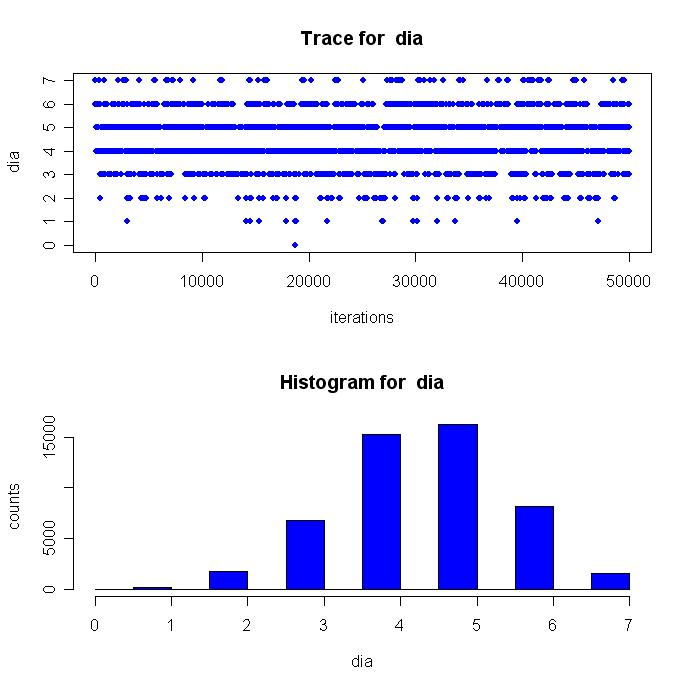
\includegraphics[width=3.5in,height=3.5in]{images/dia.jpg}
\caption {Plot of the Markov Chain Produced for the \code{dia}
Parameter in the UTI Example}
\end{center}
\end{figure}

The estimated conditional distribution of the sufficient statistic
for \code{dia} shown in the histogram is stored in the
``\code{elrm}" object and may be displayed by typing
\begin{CodeChunk}
\begin{CodeInput}
R> uti.elrm$dis
\end{CodeInput}
\begin{CodeOutput}
$dia
     dia         freq
[1,]   0 0.0001428571
[2,]   1 0.0032040816
[3,]   7 0.0303061224
[4,]   2 0.0360000000
[5,]   3 0.1350816327
[6,]   6 0.1638367347
[7,]   4 0.3051836735
[8,]   5 0.3262448980
\end{CodeOutput}
\end{CodeChunk}

\subsection{Hypothetical Drug Experiment Example}
The drugDat dataset from the \pkg{elrm}, shown below,
can be loaded into \proglang{R} with the
command:
\begin{CodeInput}
R> data("drugDat")
\end{CodeInput}
These simulated data are for a hypothetical drug experiment
comparing control versus treatment. The response variable,
\code{recovered}, indicates whether or not the patient recovered
from a given condition. The covariates of interest are \code{sex}
(1=male, 0=female) and \code{treatment} (1=treatment, 0=control).
\begin{CodeChunk}
\begin{CodeInput}
R> drugDat
\end{CodeInput}
\begin{CodeOutput}
  sex treatment recovered  n
1   1         1        16 27
2   0         1        10 19
3   1         0        13 32
4   0         0         7 21
\end{CodeOutput}
\end{CodeChunk}
For a rough assessment, based on only 2000 Markov chain
iterations, of whether the effects of \code{sex} and
\code{treatment} are jointly significant, we could call the
\code{elrm()} method as follows.
\begin{CodeChunk}
\begin{CodeInput}
R> drug.elrm <- elrm(formula = recovered/n ~ sex + treatment,
interest = ~sex + treatment, iter = 2000, dataset = drugDat)
\end{CodeInput}
\begin{CodeOutput}
Generating the Markov chain ...
Progress: 100%
Generation of the Markov Chain required 1 secs
Conducting inference ...
Warning messages:
1: 'sex' extracted sample is too small for inference (less than 1000)
2: 'treatment' extracted sample is too small for inference (less than 1000)
Inference required 0 secs
\end{CodeOutput}
\end{CodeChunk}
The warnings indicate that full conditional inference for
\code{sex} and \code{treatment} will be unreliable because the
extracted Markov chains are too small. Whenever full conditional
inference for a parameter is based on an extracted Markov chain of
length less than 1000, \pkg{elrm} will print a warning message and
will not return the associated results. Applying the
\code{summary()} method, we obtain:
\begin{CodeChunk}
\begin{CodeInput}
R> summary(drug.elrm)
\end{CodeInput}
\begin{CodeOutput}
Call:
[[1]]
elrm(formula = recovered/n ~ sex + treatment,
     interest = ~sex + treatment, iter = 2000,
     dataset = drugDat)

Results:
          estimate p-value p-value_se mc_size
joint           NA   0.097     0.0141    2000
sex             NA      NA         NA      69
treatment       NA      NA         NA     240

95% Confidence Intervals for Parameters

          lower upper
sex          NA    NA
treatment    NA    NA
\end{CodeOutput}
\end{CodeChunk}
To obtain results for full conditional inference on the separate
effects of \code{sex} and \code{treatment}, we may try augmenting
the Markov chain with a call to \code{update()}. For example, we
could increase the length of the chain by 50,000 iterations (from
2000 to 52,000) and use a burn-in period of 5000:
\begin{CodeChunk}
\begin{CodeInput}
drug.elrm <- update(drug.elrm, iter = 50000, burnIn = 5000)
\end{CodeInput}
\begin{CodeOutput}
Generating the Markov chain ...
Progress: 100%
Generation of the Markov Chain required 24 secs
Conducting inference ...
Inference required 6 secs
\end{CodeOutput}
\end{CodeChunk}
Once the \code{update()} is complete, applying the \code{summary()} method
gives the following results:
\begin{CodeChunk}
\begin{CodeInput}
R> summary(drug.elrm)
\end{CodeInput}
\begin{CodeOutput}
Call: [[1]] elrm(formula = recovered/n ~ sex + treatment,
                 interest = ~sex + treatment, iter = 2000,
                 dataset = drugDat)

[[2]] update.elrm(object = drug.elrm, iter = 50000, burnIn = 5000)

Results:
          estimate p-value p-value_se mc_size
joint           NA 0.15319    0.00290   47000
sex        0.30934 0.54259    0.01499    1397
treatment  0.75603 0.07359    0.00481    6305

95% Confidence Intervals for Parameters

               lower    upper
sex       -0.6048941 1.292658
treatment -0.1285475 1.866684
\end{CodeOutput}
\end{CodeChunk}
The estimated exact p-value for the joint effect of \code{sex} and
\code{treatment} and its Monte Carlo standard error are based on a
Markov chain of length 47,000 (after a burn-in of 5000). Full
conditional inferences for \code{sex} and \code{treatment} are
based on the shorter extracted Markov chains of length 1397 and
6305, respectively.

\section{Evaluation} \label{Evaluation}

In this section we compare the results obtained by \pkg{elrm} and
\pkg{LogXact} for the urinary tract infection data and the
hypothetical drug experiment data.

\subsection{Urinary Tract Infection Example}

Exact inference for the \code{dia} parameter could not be obtained
by \pkg{LogXact}~7 due to memory constraints, while the Gibb's
sampler `MCMC' option produced a degenerate chain. However, the
`Monte Carlo' approximate exact method in \pkg{LogXact}~7 was able
to conduct the inference. The \pkg{LogXact}~7 results were
obtained using the default setting (10,000 independent
observations) for the Monte Carlo method, which took 10 minutes to
complete and required a cumbersome 1042 MB of memory. In contrast,
\pkg{elrm} took 4.6 minutes to produce a chain of 50,000 dependent
observations and required only 75 MB of memory.

Inferences for the \code{dia} regression parameter obtained by
\pkg{LogXact}~7 and \pkg{elrm} are shown in Table \ref{inference
for dia}, and are similar.
\begin{table}[h!]
\begin{center}
\begin{tabular}{ccccc}
& estimate & 95\% CI & p-value & SE of p-value \\
\cline{2-5}\cline{4-5} \multicolumn{1}{l}{\code{dia}
(\pkg{LogXact}~7)} & \multicolumn{1}{|c}{2.0500 MUE} &
\multicolumn{1}{|c|}{(-0.0726, +INF)} &
\multicolumn{1}{|c}{0.0298} & \multicolumn{1}{|c|}{0.0033} \\
\cline{2-5}\cline{4-5} \multicolumn{1}{l}{\code{dia} (\pkg{elrm})}
& \multicolumn{1}{|c}{1.9640 MUE} & \multicolumn{1}{|c|}{(-0.0763,
+INF)} &
\multicolumn{1}{|c}{0.0337} & \multicolumn{1}{|c|}{0.0057} \\
\cline{2-5}\cline{4-5}
\end{tabular}
\end{center}
\label{inference for dia} \caption{Inference for the \code{dia}
Parameter in the UTI Example}
\end{table}
However, as shown in Table \ref{emprical dist. dia}, some
differences may be observed in the corresponding conditional
distributions estimated by each method. A noticeable difference is
that \pkg{LogXact}~7 does not sample the value zero, suggesting
that the \pkg{elrm} Markov chain mixed well.
\begin{table}[h!]
\begin{center}
\begin{tabular}{lcc}
\code{dia} & \pkg{elrm} &  \ \pkg{LogXact}~7 \\ \hline
0 & \multicolumn{1}{|c}{ \ 0.0001} &  \ -- \\
1 & \multicolumn{1}{|c}{ \ 0.0032} &  \ 0.0013 \\
2 & \multicolumn{1}{|c}{ \ 0.0360} &  \ 0.0115 \\
3 & \multicolumn{1}{|c}{ \ 0.1351} &  \ 0.0693 \\
4 & \multicolumn{1}{|c}{ \ 0.3052} &  \ 0.2224 \\
5 & \multicolumn{1}{|c}{ \ 0.3262} &  \ 0.4566 \\
6 & \multicolumn{1}{|c}{ \ 0.1638} &  \ 0.2219 \\
7 & \multicolumn{1}{|c}{ \ 0.0303} &  \ 0.0170%
\end{tabular}
\end{center}
\label{emprical dist. dia} \caption{Empirical Conditional
Distribution of the Sufficient Statistic for the \code{dia}
Parameter in the UTI Example}
\end{table}

\subsection{Hypothetical Drug Experiment Example}

The results obtained by \pkg{elrm} for the \code{drugDat} dataset
are summarized in Table \ref{elrm/logxact results drugDat}. Also
included in Table \ref{elrm/logxact results drugDat} are the exact
results obtained by \pkg{LogXact}~7 and the absolute relative
error between the \pkg{elrm} and \pkg{LogXact}~7 results. The
\pkg{elrm} results are in close agreement with those produced by
\pkg{LogXact}~7's exact method.

\begin{table}[h!]
\begin{center}
\begin{tabular}{|c|c|l|c|l|c|l|}
\hline & \multicolumn{2}{|c|}{\pkg{elrm}} &
\multicolumn{2}{|c|}{\pkg{LogXact}~7} &
\multicolumn{2}{|c|}{relative error} \\ \cline{2-7}
\multicolumn{1}{|l|}{} & estimate & p-value & estimate & p-value &
estimate & p-value \\ \hline \multicolumn{1}{|l|}{joint} & -- &
\multicolumn{1}{|r|}{0.1532} & \multicolumn{1}{|c|}{--} &
\multicolumn{1}{|r|}{0.1409} & -- & \multicolumn{1}{|r|}{0.0872} \\
\hline \multicolumn{1}{|l|}{\code{sex}} &
\multicolumn{1}{|r|}{0.3093} & \multicolumn{1}{|r|}{0.5426} &
\multicolumn{1}{|r|}{0.2862} & \multicolumn{1}{|r|}{0.5371} &
\multicolumn{1}{|r|}{0.0809} & \multicolumn{1}{|r|}{0.0102} \\
\hline \multicolumn{1}{|l|}{\code{treatment}} &
\multicolumn{1}{|r|}{0.7560} & \multicolumn{1}{|r|}{0.0736} &
\multicolumn{1}{|r|}{0.7559} & \multicolumn{1}{|r|}{0.0720} &
\multicolumn{1}{|r|}{0.0002} & \multicolumn{1}{|r|}{0.0221} \\
\hline
\end{tabular}
\end{center}
\label{elrm/logxact results drugDat} \caption{Comparison of
\pkg{elrm} and \pkg{LogXact}~7 Results for the Hypothetical Drug
Experiment Data Set}
\end{table}

The percentage errors, obtained by multiplying the relative errors
by $100\%$, are all less than 10 percent, which is quite good
given that the Markov chain was moderately small with a length of
52,000 and that full conditional inference for \code{sex} and
\code{treatment} was based on relatively short Markov chains of
length 1397 and 6305, respectively.

\section{Summary} \label{Summary}

Exact conditional inference is based on the distribution of the
sufficient statistics for the parameters of interest given the
observed values of the sufficient statistics for the remaining
nuisance parameters. When data are sparse and asymptotic
approximations based on the unconditional likelihood are
unreliable, exact inference can still be made. We consider exact
conditional inference for logistic regression models.  Commercial
software packages such as \pkg{LogXact} and \pkg{SAS} require
large amounts of computer memory to make such inference from large
data sets.
%%% New
As pointed out by a reviewer, during the review of this
manuscript, the commercial software package \pkg{Stata}~10 was
released with a new command \code{exlogistic} that performs exact
inference for logistic regression models faster than
\pkg{LogXact}. However, \code{exlogistic} was unable to make
inference for the larger urinary tract infection (UTI) and
diabetes data sets used in our examples. (For the smaller data set
from the hypothetical drug experiment, however, \code{exlogistic}
gave similar results to the corresponding procedure in
\pkg{LogXact}.) To allow exact-like inference from larger data
sets, such as the UTI and diabetes data sets, we have
%%% end New
developed \pkg{elrm}, an \proglang{R} package for
conducting approximate exact inference in logistic regression
models.
The Markov chain Monte Carlo algorithm implemented in
\pkg{elrm} extends the algorithm proposed by \citet{Forster:2003}
to enable its application to large data sets. The extensions we
make relax the potential enumeration and memory constraints of
their algorithm and should enhance mixing of the chain.

Users of \proglang{R} should find \pkg{elrm} easy to work with. The
logistic model and parameters of interest are specified using
\proglang{R} formula notation similar to that of \code{glm}. Three
input arguments upon which the \pkg{elrm} algorithm depends are
the number of iterations of the Markov chain (default \code{iter}=1000),
the burn-in period (default \code{burnIn}=0) and the
value of the Markov chain mixing parameter (default \code{r}=4).
Large values of the mixing parameter \code{r} correspond to larger,
less frequent transitions in the Markov chain, while smaller values of
\code{r} correspond to smaller, more frequent transitions in the
chain. Typical values of \code{r} recommended by \citet{Forster:2003}
are 4, 6 or 8. Inference
provided by \pkg{elrm} includes an approximate exact p-value for
jointly testing that the parameters of interest are equal to zero,
an approximate exact p-value for separately testing each parameter
of interest is equal to zero, the Monte Carlo standard error of
each reported p-value, and point and interval estimates of the
coefficients of interest in the logistic regression model.

\section*{Acknowledgements}
We would like to thank {\AA}ke Lernmark,
the Swedish Childhood Diabetes Study Group and the
Diabetes Incidence in Sweden Study Group for
providing access to the diabetes data that motivated this work.
Thanks also to a referee for helpful comments.
This research was supported
by Natural Sciences and Engineering Research Council of Canada grants
227972-00 and 213124-03,
by Canadian Institutes of Health Research grants
NPG-64869 and ATF-66667, and in part by
the Mathematics of Information Technology and Complex Systems,
Canadian National Centres of Excellence.
JG is a Scholar of the Michael Smith Foundation for Health Research.

\bibliography{biblio}
\nocite{*}


\end{document}
